\subsection{Stochastic Algorithm}
\label{subsec:03:salgo}

The first algorithm described by \citeauthor{tsiligiridis_heuristic_1984} is the \emph{Stochastic Algorithm} (S-Algorithm).
It starts at the start node and iteratively constructs a path by randomly choosing an available node in each step.
The nodes are not chosen \emph{uniformly} at random. Rather, each node's probability of being chosen depend on a calculated desirability value which will be defined shortly.
If at any point, the only available node is the end node, it is included as the last node of the path and the algorithm terminates.

To recount, $G = (V, E)$ is a complete Euclidean graph with $n := |V|$.
$s(v_i)$ refers to the score of node $v_i \in V$, whereas $t(v_i,v_j)$ refers to the weight of the edge $\{v_i, v_j\}$ for $1 \leq i \neq j \leq n$.
$v_1 \in V$ is the start node and $v_n \in V$ the end node.
However, there are some more variables required by this algorithm.

Let $last \in V$ refer to the last node visited by the algorithm in its previous step.
A node $v_i \in V$ is considered to be \emph{available} if and only if it has not been visited yet and adding it to the current path would not violate $T_{max}$ when adding the distances $t(last, v_i)$ and $t(v_i, v_n)$. (akin to the example in \cref{subsec:02:triangle}) 
The end node $v_n$ is excluded from this, however.
Then let $A \subset V$ be the set of currently available nodes. 
Let $r \in \mathbb{R}_+$ be a parameter used to scale the desirability value exponentially.

Then the desirability value $D(v_i)$ for every $v_i \in A$ is defined as follows:

\begin{align*}
    D(v_i) := \left( \frac{s(v_i)}{t(last, v_i)} \right)^r
\end{align*}

This value aims to provide a measure for how valuable a node is estimated to be when included in the path.
The last parameter we will use is $1 \leq l \in \mathbb{N}$ which represents the maximum number of available nodes we want to consider in each iteration when choosing a node at random.
We only consider the $l$ most desirable nodes.

So to in short summarize the algorithm, we initialize the path with only $v_1$ and $A = V / \{v_1, v_n\}$.
We update $A$ by checking all nodes $v_i \in A$ whether adding $v_i$ would violate $T_{max}$ and removing those that do. 
We calculate all desirability values $D(v_i)$ for the remaining elements in $A$ and take the $k$ most desirable nodes from $A$ where $k := \min(l, |A|)$. Let $A'$ be the set of these nodes.
For each of these nodes $v_i \in A'$ the probability of being chosen is equal to:
\begin{align*}
    \frac{D(v_i)}{\sum_{j=1}^k D(v_j)}
\end{align*}
Choose a node according to these probabilities, insert it into the path and repeat the process (save for the initialization).

\begin{wrapfigure}{r}{5cm}
    \centering
    \scalebox{0.9}{
        \begin{tikzpicture}[vertex/.style={draw}]
            \node at (1, 2.2) {$T_{max}=4$};
            \node at (-1,0) (invis) {};
            \node[vertex, red] at (0,0) (0) {$0$};
            \node[vertex] at (2,0) (1) {$0$};
            \node[vertex, blue] at (1,1) (2) {$4$};
            \node[vertex, blue] at (1,-1) (3) {$6$};
            \node at (3,0) (invis2) {};

            \node[blue] at (1,1.6) {$\tfrac{4}{7}$};
            \node[blue] at (1,-1.6) {$\tfrac{3}{7}$};

            \draw[->, red] (invis) -- (0);
            \draw (0) -- node[above left] {$1$} (1);
            \draw[blue] (0) |- node [below right] {$1$} (2);
            \draw[blue] (0) |- node [above right] {$2$} (3);
            \draw (2) -- (3);
            \draw (2) -| node [below left] {$2$} (1);
            \draw (3) -| node [above left] {$2$} (1);
            \draw[->] (1) -- (invis2);
        \end{tikzpicture}
    }
    \caption{The S-Algorithm at work.}
    \label{fig:03:salgoexample}
\end{wrapfigure}

A small example is illustrated in \cref{fig:03:salgoexample}.
The number inside a node is its score. 
The blue-colored nodes are available nodes that the algorithm is considering and the numbers besides the blue nodes are the probabilities of this node being chosen.
Elements that are currently part of the path are colored red.

There are other elements in these equations in the original paper not covered here.
However, as noted by \citeauthor{tsiligiridis_heuristic_1984}, these other values did not contribute to the quality of the solution in his evaluations, so they are omitted here. 

\subsubsection{Generalizing to non-Euclidean inputs}

The inputs in \citeauthor{tsiligiridis_heuristic_1984}' paper are Euclidean, and his descriptions are formulated in respect to a Euclidean input.
However, the algorithm does not explicitly require the graph to have any particular properties except for every node to be directly connected to the end node $v_n$.
The reason for this is that the algorithm considers a node $v_i$ to be available if the path can move from the last visited node to $v_i$ and from $v_i$ to $v_n$ without violating $T_{max}$.

\begin{wrapfigure}{l}{5.5cm}
    \centering
    \scalebox{0.9}{
        \begin{tikzpicture}[vertex/.style={draw}]
            \node at (-1,0) (invis) {};
            \node[vertex] at (0,0) (0) {$v_0$};
            \node[below=0mm of 0] (w0) {$0$};
            \node[vertex] at (0,2) (1) {$v_1$};
            \node[above=0.5mm of 1] (w1) {$10$};
            \node[vertex] at (2,2) (2) {$v_2$};
            \node[above=0.5mm of 2] (w2) {$5$};
            \node[vertex] at (2,0) (3) {$v_3$};
            \node[below=0.5mm of 3] (w3) {$0$};
            \node at (3,0) (invis2) {};

            \draw[->] (invis) -- (0);
            \draw (0) -- node[left] {$1$} (1);
            \draw (1) -- node[above] {$1$} (2);
            \draw (2) -- node[right] {$1$} (3);
            \draw (0) -- node[below] {$5$} (3);
            \draw (0) -- node[left] {$3$} (2);
            \draw (1) -- (3);

            \draw[->] (3) -- (invis2);

            \node at (1, 3) {$T_{max}=3$};
        \end{tikzpicture}
    }
    \caption{An example that illustrates that the S-Algorithm can fail to find a path even in very simple graphs not fulfilling the triangle equation.}
    \label{fig:03:salgofailexample}
\end{wrapfigure}

\phantomsection
\label{par:03:salgotriangle}
\paragraph{Triangle Inequality} 
As explained in \cref{subsec:02:triangle}, for this heuristic to work, the graph should satisfy the triangle inequality.
Otherwise, it would not be possible to decide whether a constraint-respecting path can be found when including a specific vertex; at least not in the way this algorithm does it.
If the graph does not satisfy the inequality, this might lead the algorithm to miss pursuing paths that might be profitable,
or might even lead to the algorithm not being able to find a path even in very small graphs. 

This is illustrated in \cref{fig:03:salgofailexample}. The obvious optimal path is the path taking all the edges with weight $1$.
However, $v_1$ has a weight $3$ edge to the end node and $v_2$ has a weight $3$ edge leading to it.
If any of these nodes were added to the path, they would lead to a path cost of $4$ (remember that we include the cost of the edge from $v_1$ or $v_2$ to the end node $v_3$), violating $T_{max} = 3$.
In addition, since the edge between the start and end node has a weight of $5$, this edge cannot be taken either.
As a result, the algorithm will not consider any nodes to be available and output that no path was found.
This result is obviously incorrect.

\paragraph{Inserting $\infty$ Edges} 
As alluded to before in \cref{subsec:02:complete}, one can make a graph complete by inserting missing edges with a weight of $\infty$.
This however, would violate the triangle inequality.
The algorithm would also ignore \emph{all} nodes $v_i$ with an $\infty$-edge to the end node $v_n$, since the edge $\{v_i, v_n\}$ could never be traversed, unless $T_{max} = \infty$.
But in this case there is no problem to solve.
One can easily imagine a graph with three nodes $A, B, C$ and edges $\{A, B\}$ and $\{B, C\}$, each having a respective finite weight $x$ and $y$.
If we were to complete this graph by inserting the edge $\{A, C\}$ with a weight of $\infty$, then $t(A, B) + t(B,C) = x + y < \infty = t(A, C)$
which is an obvious violation of the triangle inequality.

As a result, this algorithm can work correctly on complete graphs which satisfy the triangle inequality with none of its functionality being hampered.
However, other graphs would likely result in suboptimal results. 
